\externaldocument{GEP/deliverable1.tex}

\section{Integración de OmpSs-2 en C/C++ COMPSs}

Con tal de realizar una buena integración necesitamos conocer bien cómo funcionan y/o cómo están hechos los componentes a integrar. Con tal de adquirir los conocimientos necesarios, vamos a indagar en la estructura interna del \textit{binding} de \textit{C/C++} de \textit{COMPSs} y a entender cómo se desarrolla y compila una aplicación. También deberemos ver cómo funciona la \textit{API} del \textit{runtime} de \textit{OmpSs-2} \textit{Nanos6} y el proceso habitual de desarrollo y compilado de una aplicación que utiliza el modo librería.

\subsection{Estructura de los bindings}

El \textit{runtime} de \textit{COMPSs} fue desarrollado en \textit{Java}, por lo que si queremos soportar cualquier lenguaje (salvo el propio \textit{Java}), necesitamos de alguna manera establecer comunicación con ese lenguaje. Es decir, necesitaremos un mecanismo que nos permita ejecutar código de este lenguaje a soportar, por supuesto, en ambas direcciones. 
\par\bigskip
Actualmente, \textit{COMPSs} cuenta con los \textit{bindings} de \textit{C/C++} y \textit{Python} (usualmente conocido como \textit{PyCOMPSs}), que utilizan estos mecanismos descritos anteriormente. Para efectuar la ejecución entre \textit{Java} y \textit{C/C++} se utiliza la \textit{Java Native Interface}, dado que desde \textit{Python} se puede utilizar la \textit{Python-C API} para , con un componente intermedio entre \textit{Python} y \textit{Java} escrito en \textit{C/C++} (utilizando la \textit{JNI}) permitiríamos efectuar llamadas desde \textit{C/C++} y \textit{Python} al \textit{runtime} y al revés. 
\par\bigskip
La siguiente imagen muestra la estructura general de los \textit{bindings} actuales. Las cajas representan componentes de la arquitectura, el color de cada caja ha sido escogido para representar un lenguaje, por lo que dos cajas del mismo color que estén conectadas directamente con un flecha no requieren de mecanismos adicionales.

\begin{figure}[H]
    \centering 
    \caption{Estructura de los bindings de COMPSs.}
    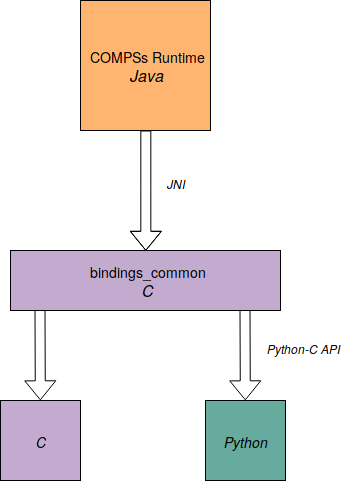
\includegraphics[scale=0.6]{estructuraBindings.png}
    \label{fig:estructura_bindings}
\end{figure}

\subsection{Modelo de ejecución en el binding C/C++}

\textit{C} y \textit{C++} son lenguajes de programación compilados, esto quiere decir que necesitamos un segundo programa llamado compilador que procese nuestro programa y genere un fichero que nuestro ordenador pueda ejecutar, a este proceso se le llama compilar y al fichero generado, binario. De esta manera, para poder obtener el modelo de ejecución introducido en la sección \ref{modeloejecucion}, necesitaremos compilar dos binarios, uno para el \textit{master} y otro para los \textit{workers}.
\par\bigskip

\begin{comment}
La aplicación que desarrolla el usuario, \textit{a priori} no envía las tareas a ejecutar ni las dependencias entre estas, no gestiona el \textit{runtime}, pero es desarrollada siguiendo unas directrices que nos permitirán generar código que sí gestione todo lo que es necesario con tal de que la aplicación se distribuya correctamente. 
\end{comment}

La aplicación que desarrolle el usuario, tiene que ser transparente al \textit{runtime}, para conseguirlo tan sólo se necesita una interfaz indicando las tareas a detectar al ejecutar la aplicación. Entonces, una vez compilemos la aplicación de COMPSs en C/C++, se generará automáticamente (a partir de ahora \textit{autogenerar}) código para las tareas, que gestionarán la comunicación con el \textit{runtime}.
\smallskip
La siguiente imagen describe de manera visual cómo se compila una aplicación. 

\begin{figure}[H]
    \centering 
    \caption{Proceso de compilación de una aplicación COMPSs C/C++.}
    %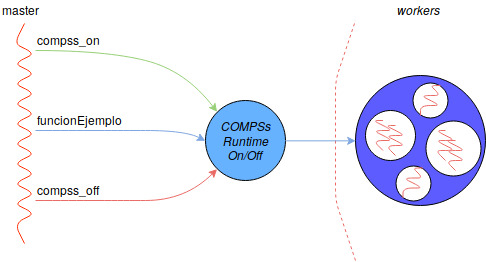
\includegraphics[width=\textwidth]{sta-masterworker.jpg}
    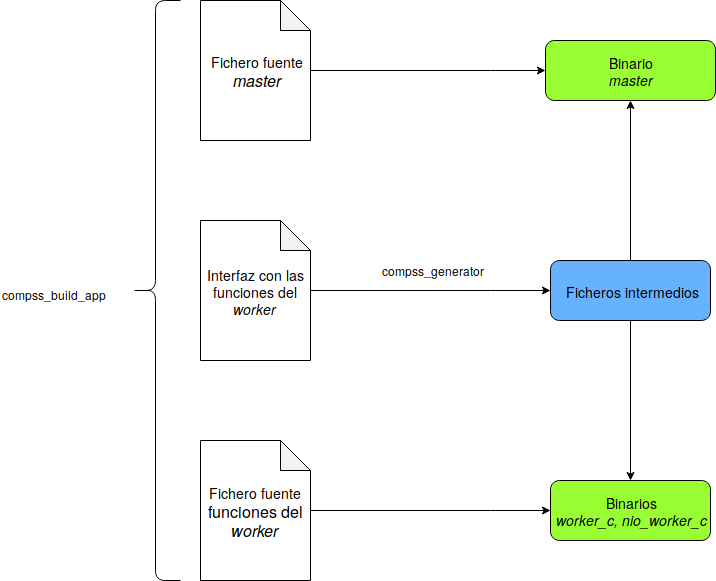
\includegraphics[scale=0.6]{workflowCompilado.png}
    \label{fig:workflowcompilado}
\end{figure}

\par\bigskip
Para facilitar el compilado de la aplicación se utiliza el script \textit{compss\_build\_app}, y para hacer la generación de código a partir de la interfaz, el binario \textit{compss\_generator}.
La aplicación una vez desarrollada por el usuario, compilada sin \textit{COMPSs} por el medio también funcionaría, pero sencillamente las tareas serían ejecutadas \textit{in situ} en el \textit{master}.  Lo que pretendemos hacer al introducir \textit{COMPSs} es que el \textit{master}, en vez de ejecutar la tarea, comunique al \textit{runtime} que se debe ejecutar una tarea, y este se encargue de ejecutarla en un \textit{worker}, todo evidentemente, de manera transparente al usuario.
\par\bigskip

\bigskip
En la figura \ref{fig:workflowcompilado} veíamos la caja negra de ficheros intermedios, estos ficheros son el \textit{stubs} y \textit{executor} (siempre del estilo, \textit{ejemplo-stubs.cc} y \textit{ejemplo-executor.cc} donde ejemplo es el nombre de la aplicación compilada). El fichero \textit{stubs} corresponde con la parte del \textit{master} que se encargará de comunicarse con el \textit{runtime} para registrar la tarea. Esto lo consigue implementando las funciones de las tareas con el código para gestionar su registro, es decir, sustituyendo el código que sería propio de la ejecución de cada tarea por un código para efectuar el registro en el \textit{runtime}. Una vez registrada la tarea, eventualmente el \textit{runtime} designará a un \textit{worker} a ejecutarla. El \textit{worker} recibirá la tarea que debe ejecutar, los datos necesarios y más parámetros, el \textit{executor} ha sido \textit{autogenerado} con el código principal de la aplicación, por lo que conoce como gestionar los datos y parámetros recibidos para ejecutar la tarea pertinente. 

\begin{figure}[H]
    \centering  
    \caption{Registro y ejecución de tareas en una aplicación COMPSs C/C++.}
    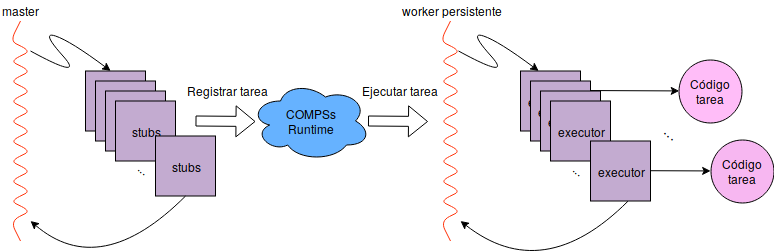
\includegraphics[scale=0.6]{stubs-executor.png}
    \label{fig:stubs-executor}
\end{figure}

La imagen anterior muestra las llamadas a funciones pertinentes a \textit{stubs} que contienen el código para registrar las tareas en el \textit{runtime}, la eventual ejecución de las tareas registradas en los \textit{workers} que hayan disponibles y como toma parte su ejecución mediante el \textit{executor}.













